\documentclass{article}
%\usepackage{geometry}
% \geometry{top = 1in, bottom = 1in, left = 1in, right = 1in}
\usepackage[top = 0.7in, bottom = 0.7in, left = 0.7in, right = 0.7in]{geometry}
\usepackage{amsmath,amssymb,amsthm,mathrsfs}
\usepackage{graphicx}
\usepackage{bm}
\usepackage{float}
\usepackage[font=footnotesize,labelfont=bf]{caption}

\usepackage{fancyhdr}
\pagestyle{fancy}
\rhead{\footnotesize {February 2018; MESA version xxxx} }
\chead{\footnotesize {Authors: } }
\lhead{\footnotesize {mesa/star/test\_suite/1.5M\_with\_diffusion} }

\begin{document}
	
	\begin{center}
		\begin{Large}
		       \textbf{1.5M WITH DIFFUSION}\\
		\end{Large}
	\end{center}

        This test is to show the capability of \texttt{MESA} to treat 	atomic diffusion during stellar evolution.  It evolves a 1.5 $M_\odot$ star from the zero age main sequence (ZAMS) to the terminal age main sequence (TAMS), or more precisely in this case, to the point when central hydrogen mass fraction drops below 0.01 (\texttt{xa\_central\_lower\_limit\_species(1) = 'h1' ; xa\_central\_lower\_limit(1) = 0.01}).\\
        
        The inlist used to produce the starting zams model (inlist\_to\_ZAMS) is provided.\\

        The convective boundaries are determined using the Ledoux criterion and predictive mixing (see MESAIV paper).\\
        
        
        There are many variables to control diffusion, and they are all listed in \texttt{mesa/star/defaults/controls.defaults} (see also the mesa web site http://mesa.sourceforge.net/controls\_defaults.html\#element\_diffusion).  To allow diffusion, the inlist for this test case sets \texttt{do\_element\_diffusion = .true.}.  It also sets a range on temperatures in which diffusion is allowed: \texttt{diffusion\_T\_full\_on = 1d3 ; diffusion\_T\_full\_off = 1d3}.  This means that diffusion is turned fully on for temperatures above 1000 K, which in this case is the whole star.  Diffusion-allowed regions can also be set by X, Y, and gamma.  There are also diffusion controls for tolerance (\texttt{diffusion\_atol = 1d-4 ; diffusion\_rtol = 1d-3}), timesteps (\texttt{diffusion\_dt\_limit = 7d11}), and ionization (\texttt{diffusion\_calculates\_ionization = .true.}).\\

        Because diffusion calculation for each individual species would be computationally intensive, \texttt{MESA} groups species into classes for diffusion computation.  Each class is given a `representative' and an `A\_max'.  This test case has five classes, with `representative' and `A\_max' listed for each respectively:  \texttt{`h1', 2 ; `he3', 3; `he4', 4 ; `o16', 16 ; `fe56', 10000}.  Each species is placed in the first class, in ascending order, that has `A\_max' greater than, or equal to, the species' atomic mass number.  Therefore, hydrogen and deuterium would go in \texttt{`h1'}, carbon, nitrogen, and oxygen would go in \texttt{`o16'}, and anything heavier would go in \texttt{`fe56'}.\\

  We illustrate some results in the figure below. Those were obtained using better time and mesh resolution than in the test\_suite inlist, namely \texttt{max\_years\_for\_timestep= 5d5} and \texttt{mesh\_delta\_coeff = 0.5}.\\
       
For speed purposes the values used in the inlist of the test\_suite example for the maximum allowed timestep and the mesh size do not produce completely converged models.  A convergence study should be done when using this inlist for science purposes.\\       

\pagebreak
        
          In the figure below we show the profiles of the abundances in the star at the end of the run. The dashed lines are the results obtained when the diffusion is turned off  (\texttt{do\_element\_diffusion = .false.}). The results obtained when diffusion is set to  \texttt{do\_element\_diffusion = .true.} are shown in plain lines. The effects of diffusion on the mass fractions are clearly seen in this figure.  At the surface of the star, the heavy elements sink while the surface is enriched in hydrogen due to diffusion.  Diffusion also smoothes the composition gradients at the top of the convective core.       
                  
	\begin{figure}[H]
                \begin{minipage}[t]{0.5\linewidth}
		       \centering
		       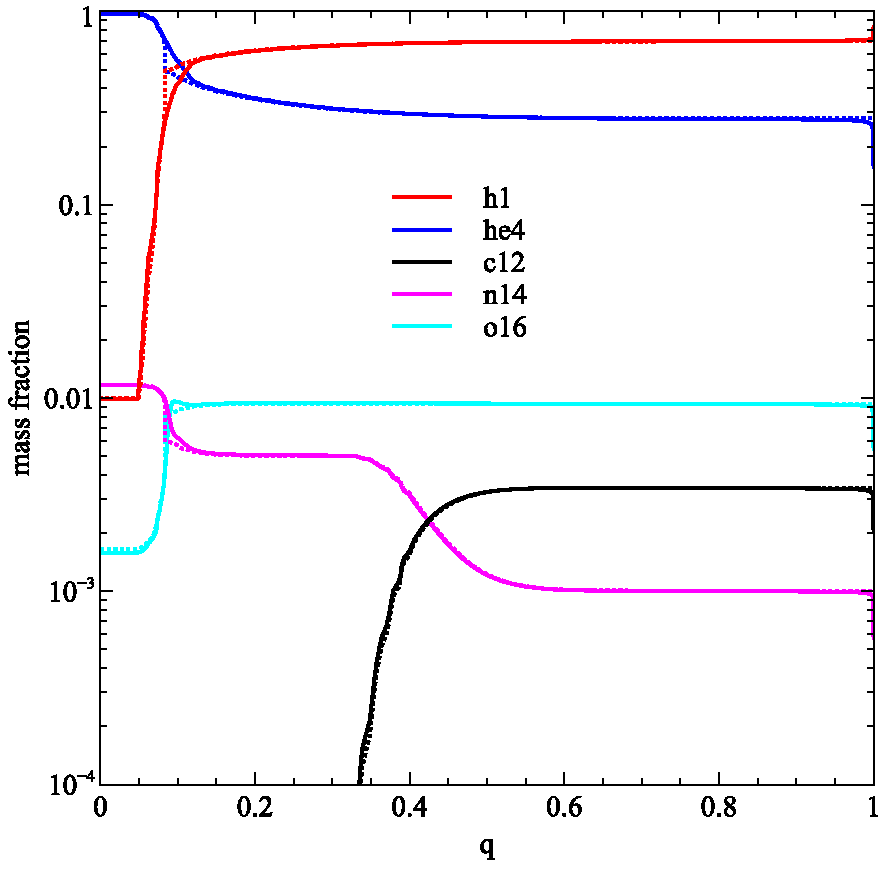
\includegraphics[width = 3.5in]{fig.pdf}
		       \caption{Abundance profiles, with (plain lines) and without (dotted lines) diffusion.}
		       \label{fig:1}
                \end{minipage}
                \hspace{0cm}
                \begin{minipage}[t]{0.5\linewidth}
                       \centering
                       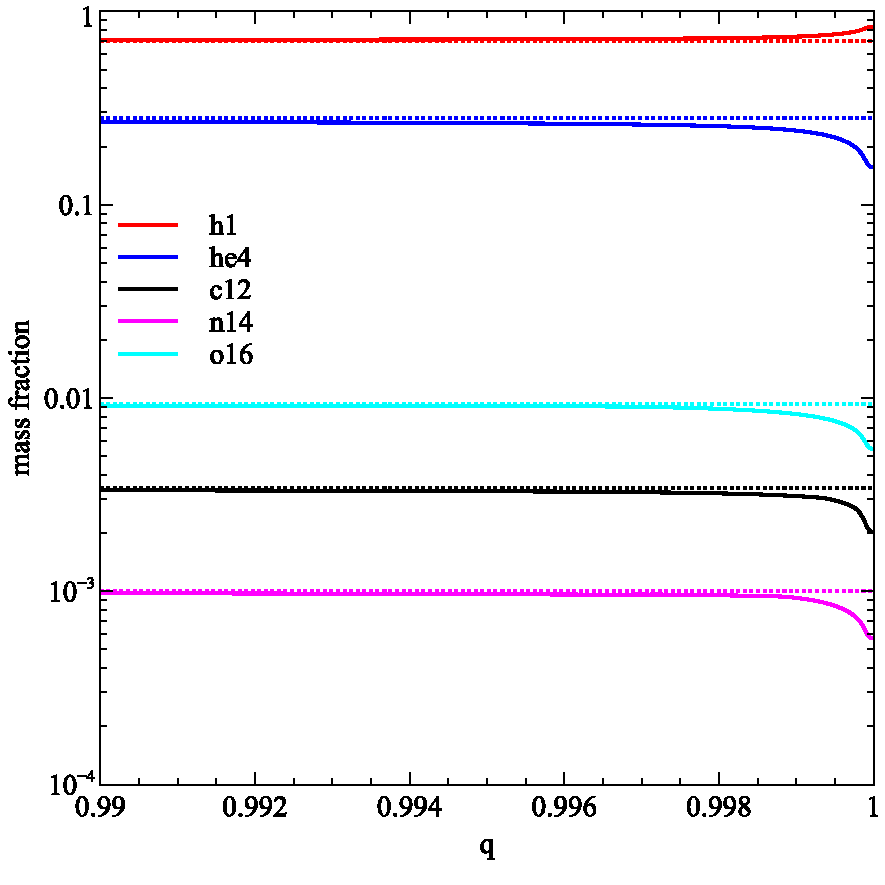
\includegraphics[width = 3.5in]{figzoom.pdf}
                       \caption{Same as figure 1 but zoom on the surface of
                        the star.}
                       \label{fig:2}
                \end{minipage}
	\end{figure}


 
 
       
\end{document}


